%% 
%% Copyright 2007, 2008, 2009 Elsevier Ltd
%% 
%% This file is part of the 'Elsarticle Bundle'.
%% ---------------------------------------------
%% 
%% It may be distributed under the conditions of the LaTeX Project Public
%% License, either version 1.2 of this license or (at your option) any
%% later version.  The latest version of this license is in
%%    http://www.latex-project.org/lppl.txt
%% and version 1.2 or later is part of all distributions of LaTeX
%% version 1999/12/01 or later.
%% 
%% The list of all files belonging to the 'Elsarticle Bundle' is
%% given in the file `manifest.txt'.
%% 

%% Template article for Elsevier's document class `elsarticle'
%% with numbered style bibliographic references
%% SP 2008/03/01
%%
%% 
%%
%% $Id: nse_preprint.tex,v 1.5 2009-11-27 20:10:38 bert Exp $
%%
%%
%\documentclass[review,12pt]{elsarticle}
\documentclass[final,3p,times,11pt]{elsarticle}
%% Use the option review to obtain double line spacing
%\documentclass[preprint,review,10pt]{elsarticle}

%% Use the options 1p,twocolumn; 3p; 3p,twocolumn; 5p; or 5p,twocolumn
%% for a journal layout:
%% \documentclass[final,1p,times]{elsarticle}
%% \documentclass[final,1p,times,twocolumn]{elsarticle}
%% \documentclass[final,3p,times]{elsarticle}
%% \documentclass[final,3p,times,twocolumn]{elsarticle}
%% \documentclass[final,5p,times]{elsarticle}
%% \documentclass[final,5p,times,twocolumn]{elsarticle}

%% if you use PostScript figures in your article
%% use the graphics package for simple commands
%% \usepackage{graphics}
%% or use the graphicx package for more complicated commands
%% \usepackage{graphicx}
%% or use the epsfig package if you prefer to use the old commands
%% \usepackage{epsfig}

%% The amssymb package provides various useful mathematical symbols
\usepackage{amssymb,graphicx,amsmath,booktabs,subfigure,bm,longtable,rotating,setspace}
\renewcommand{\thefootnote}{\aleph{footnote}}
%% natbib.sty is loaded by default. However, natbib options can be
%% provided with \biboptions{...} command. Following options are
%% valid:

%%   round  -  round parentheses are used (default)
%%   square -  square brackets are used   [option]
%%   curly  -  curly braces are used      {option}
%%   angle  -  angle brackets are used    <option>
%%   semicolon  -  multiple citations separated by semi-colon 
%%   colon  - same as semicolon, an earlier confusion
%%   comma  -  separated by comma
%%   numbers-  selects numerical citations
%%   super  -  numerical citations as superscripts
%%   sort   -  sorts multiple citations according to order in ref. list
%%   sort&compress   -  like sort, but also compresses numerical citations
%%   compress - compresses without sorting
\biboptions{super,sort&compress}

%%    Journal Name
\journal{18.086}

% OTHER DOCUMENT-SPECIFIC OPTIONS
\newcommand{\eg}{{\it e.g. }}
\newcommand{\ie}{{\it i.e. }}
\long\def\symbolfootnote[#1]#2{\begingroup%
\def\thefootnote{\fnsymbol{footnote}}\footnote[#1]{#2}\endgroup} 

\renewcommand*{\today}{May 18, 2010}

\begin{document}

\begin{frontmatter}

%% Title, authors and addresses

\title{Direct Solution of the Discrete Ordinates Equations}

%% use optional labels to link authors explicitly to addresses:
%% \author[label1,label2]{<author name>}
%% \address[label1]{<address>}
%% \address[label2]{<address>}

\author[primary]{Jeremy A. Roberts\corref{mit}}
\address[primary]{Massachusetts Institute of Technology,
                  77 Massachusetts Avenue, Cambridge, MA 02139-4307}
\cortext[mit]{email: robertsj@mit.edu}

\pagebreak

\begin{abstract}
{\small
The purpose of this paper is to investigate and implement the discrete ordinates method for one- and two-dimensional multigroup neutron transport, and to solve directly the resulting equations.  Historically, the discrete ordinates equations have been solved via the power iteration method (PI).  The approach as typically implemented is very memory efficient, but for highly diffusive problems, the PI method is notoriously ineffective.  Several techniques to accelerate the PI method have been developed, but they are complicated even for simple geometries.  Here, an alternative approach is investigated, which is to solve the discrete ordinates system directly.  The general forms of the multigroup discrete ordinates matrices in both one and two dimensions have been derived and implemented in MATLAB using its built-in sparse matrix utilities.  To solve the systems, both the standard ``backslash'' for direct elimination and combinations of built-in Krylov solvers (GMRES and BiCG-STAB) with ILU preconditioning are studied.  The computational expense for these direct approaches is compared to that of the standard PI approach, which has also been implemented in Matlab and verified against a production discrete ordinates code.  One-dimensional studies suggest that the direct approach (with either elimination or Krylov solvers) is faster than the PI method by roughly a factor of two for low angular orders (and hence small bandwidths).  For highly diffusive problems, the direct method is up to an order of magnitude faster.  In general, the efficiency of the direct method was observed to degrade for larger matrix bandwidths, which occurs for higher angular resolution and more energy groups.  Moreover, direct elimination in all cases was more efficient than the Krylov techniques investigated.  Finally, the cost of the direct method was due largely to the expense of building the underlying sparse matrix via the built-in commands; whether a more efficient way to do this in MATLAB remains a topic for continued work.}
\end{abstract}

\begin{keyword}
%% keywords here, in the form: keyword \sep keyword
neutron transport \sep discrete ordinates \sep Krylov methods
\end{keyword}

\pagebreak

\end{frontmatter}

%%
%% Start line numbering here if you want
%%
%%\linenumbers

%% main text
\section{Introduction}
\label{in}

In the computational nuclear engineering community, the neutron transport equation and methods of solving it are of extreme importance.  The equation governs physics of reactors, radiation transport through shields, and to a degree, dose deposition by neutral particles.  Of current interest are means to solve extremely large radiation transport problems on the largest parallel computers available.  Of the methods available for solving such problems, the discrete ordinates method is perhaps the oldest and most popular technique.

Historically, the discrete ordinates equations have been solved via memory-efficient ``sweeps'' inside a power iteration scheme.  This approach was necessary given the computational memory available in previous years.  On the other hand, it is now possible to form and solve the resulting linear system directly \cite{patton2002apg,swesty2006std}.  In this paper, we cast the discrete ordinates into a linear system.  To solve the system in MATLAB, we use the standard ``backslash'' for direct elimination and combinations of built-in Krylov solvers (GMRES and BiCG-STAB) with ILU preconditioning.

The rest of this paper is organized as follows.  In Section 2, the neutron transport equation and discrete ordinates approximation are described.  The standard approach as described is implemented in MATLAB and verified against the production code PARTISN.  Section 3 develops a direct approach to solving the discrete ordinates equations, and the resulting matrix forms are given.  Section 4 provides results for several one-dimensional problems, which are compared to some results of the literature.  Section 5 provides a conclusion and connects this paper with ongoing work elsewhere.

\section{Discrete Ordinates Equations}

\subsection{Neutron Transport}

  The fundamental equation governing interactions of neutral particles with matter is a linearized form of the Boltzmann equation, which we refer to as the neutron transport equation.  In its most common integro-differential form, we have

  \begin{equation}
  \begin{split} 
     \hat{\Omega} \cdot \nabla \psi &+ \Sigma_t(\vec{r},E) \psi(\vec{r},\Omega,E) = \\
         & \int_{4\pi}d\Omega' \int^{\infty}_{0}dE' \Sigma_s(\vec{r},\Omega' \to \Omega, E'\to E) \psi (\vec{r},\Omega',E') + S(\vec{r},\Omega,E) \, ,
  \end{split}
  \end{equation}
  where $\psi$ is the angular flux that essentially describes the population of neutrons in an element of the six dimensional phase space $(\vec{r},\Omega,E)$.  The probability of any interaction is quantified by the total cross-section $\Sigma_T$ and the probability of a scattering event bringing a particle from $(\vec{r},\Omega',E')$ to $(\vec{r},\Omega,E)$ is quantified by the scattering cross-section $\Sigma_S$.  $S$ serves is any external particle source.  By inspection, the neutron transport equation is a balance relation, where the left hand side is comprised of losses due to spatial leakage and collisions, and the right hand side consists of gains from in-scattering and the external source.

  The angular dependence of the neutron transport equation is unique and gives rise to much of the difficulty in obtaining analytical solutions to all but the simplest problems.  The energy dependence of the underlying data is also often very difficult, as the interaction cross-sections vary by several orders of magnitude over the seven or more orders of magnitude of energy important in nuclear engineering.

  To solve the neutron transport equation, several computational techniques exist to treat each of the variables.  To treat the energy variable, the multigroup approach is common.  The cross-sections $\Sigma$ become $\Sigma_g$, piecewise constants over $E_g$ to $E_{g-1}$.  This greatly simplifies matters, because it takes the transport equation above to a system of one-group equations.  Generating the appropriate group constants is not trivial, but any further discussion is out of the present scope.  To treat the angular variable, the two most popular approaches are moment expansions and the discrete ordinates method.  In the former approach, $\psi(x,\mu)$ (in 1-D) becomes $\sum_l \phi_l(x) P_l(\mu)$, where $\mu$ represents angles and $P_l$ are a set of orthogonal functions, typically Legendre polynomials (or in higher dimensions, the spherical harmonics).  In the discrete ordinates methods, the transport equation is solved for discrete angles, so that $\psi(x,\mu)$ becomes $\psi_n(x)$ for $\mu_n$
  and integrals over $\mu$ become weighted sums.  In this paper, we focus on this latter approach. Finally, both the finite difference and finite element methods are popular for treating the spatial variable.  In this work, we use the finite difference approach.

\subsection{Derivation of Discrete Ordinates Equations}

  Here, we derive the discrete ordinates equations.  To simplify the exposition, we focus on the one-dimensional, one-speed transport equation with isotropic scattering and source.  The derivation for higher dimensions is straightforward, and the reader is referred to the standard text by Lewis and Miller for more details \cite{lewis1993cmn}.  Hence, the transport equation becomes
  \begin{equation}
    \mu \frac{d}{dx}\psi(x,\mu) + \Sigma_T(x)\psi(x,\mu)= \frac{\Sigma_s(x)}{2} \int^1_{-1}\psi(x,\mu)d\mu + \frac{S(x)}{2} \, ,
    \label{eq:tran}
  \end{equation}
  where $\mu$ is $\cos(\theta)$ and $\theta$ is the direction of travel particles make with respect to the $x$ axis.

  In place of $\mu$, we substitute discrete values $\mu_n$ so that Eq. $\ref{eq:tran}$ becomes
  \begin{equation}
    \mu_n \frac{d}{dx}\psi_n + \Sigma_T(x)\psi_n(x) = \frac{\Sigma_s(x)}{2}  \sum^N_{j=1} w_j \psi_j(x) + \frac{S(x)}{2} \, .
    \label{eq:tranSn}
  \end{equation}
  In one spatial dimension, the $\mu_n$ are typically roots of the Legendre polynomials, $P_N(\mu)$, and the weights $w_n$ are chosen to integrate $P_j(\mu)$, $j<N$ exactly over the domain $-1 \leq \mu \leq 1$.  Quadrature sets for two and three dimensions are more complicated and serve to conserve different quantities.  The level-symmetric quadrature sets are quite popular and are well-described elsewhere \cite{lewis1993cmn}.

  To discretize in space, the grid shown in Figure \ref{fig:slab_spatial} is used.  The angular flux $\psi$ is described at cell edges for the spatial derivative and cell centers for physical quantities (like reaction rates).  Hence,
    \begin{equation}
    \begin{split}
      \mu_n \frac{\psi_{i+1/2,n}-\psi_{i-1/2,n}} {h_i} + \Sigma_{Ti}\psi_{i,n} &= \frac{\Sigma_{Si}}{2} \sum^N_{j=1} w_j \psi_{i,j} + S_{i,n} \\
			    &= Q_{i,n} \, ,
    \end{split}
    \end{equation}
    and using the ``diamond difference'' approximation,
    \begin{equation}
      \psi_{i,n} = \frac{1}{2} ( \psi_{i+1/2,n} + \psi_{i-1/2,n} ) \, ,
    \end{equation}
    we find after some algebra that
    \begin{equation}
    \begin{split}
    \psi_{i\pm1/2,n} &= \frac{1-\Sigma_{Ti}h_i/2|\mu_n|}{1+\Sigma_{Ti}h_i/2|\mu_n|} \psi_{i\mp1/2,n} + \frac{Q_{i,n} h_i}{|\mu_n|(1+h_i/2|\mu_n|)} \\
		    &= \alpha_{i,n} \psi_{i\mp1/2,n} + \beta_{i,n} Q_{i,n} \, .
    \end{split}    
    \label{eq:sweep}
    \end{equation}
    
    Eq. \ref{eq:sweep} defines a ``sweeping'' relation that propagates boundary fluxes throughout the medium.  Note, however, that the second term on the right hand side, $Q$, contains terms involving $\psi$.  Consequently, the power iteration (PI) method is often used, in which an initial guess is made for $\psi$, $Q$ is computed, and sweeps are performed.  Then $Q$ is updated, and the process repeats until $\psi$ is converged.

   \begin{figure}[ht]  
	\centering
	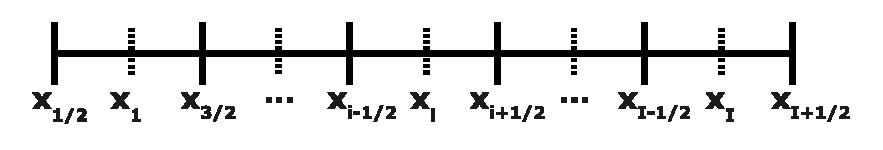
\includegraphics[keepaspectratio, width = 3.5 in]{slab_spatial}
        \caption{One-dimensional slab discretization scheme.}
        \label{fig:slab_spatial}
    \end{figure}

  While the diamond difference approach is second order accurate \cite{lewis1993cmn} and easy to implement, it can lead to locally negative angular fluxes. Other approaches for relating edge fluxes to center fluxes do exist, such as a weighted form of the diamond difference equation. Such other approaches can be more robust and avoid locally negative angular fluxes, but they are also more complicated and may not translate well into the direct solution framework to be described below.

\subsection{Code Verification}

  The discrete ordinates approach was implemented in MATLAB for both 1-D and 2-D multigroup problems using the standard power iteration method with transport sweeps.   To ensure the code produces valid results, it was compared to PARTISN for simple 1-D and 2-D problems.  PARTISN is a production-level discrete ordinates code developed at Los Alamos National Laboratory.

  The first problem is a 1-D slab of width 10 cm and uniform composition ( $\Sigma_T=1.0$ cm$^{-1}$ and $\Sigma_S = 0.5$ cm$^{-1}$).  The source is isotropic and uniformly distributed throughout the slab, and the boundary conditions are vacuum. Note, only isotropic scattering is considered (in both problems), as anisotropic scattering simply makes the data component more cumbersome while adding essentially nothing new to the mathematical approach.  Figure \ref{fig:one_d_comp} shows the scalar flux $\phi$ from both the MATLAB code and PARTISN.\footnote{Note, the scalar flux $\phi$ is the integral over all directions of the angular flux $\psi$; for the $S_N$ approximation, this is the sum $\phi_i = \sum_n w_n \psi_{in}$ for an x point $i$ and discrete direction $n$} Note, this problem used an $S_8$ approximation (\ie 8 directions), 100 spatial mesh intervals, and a (relative) pointwise convergence criteria for $\phi$ of $1\times 10^{-9}$. 

  \begin{figure}[ht] 
      \centering
      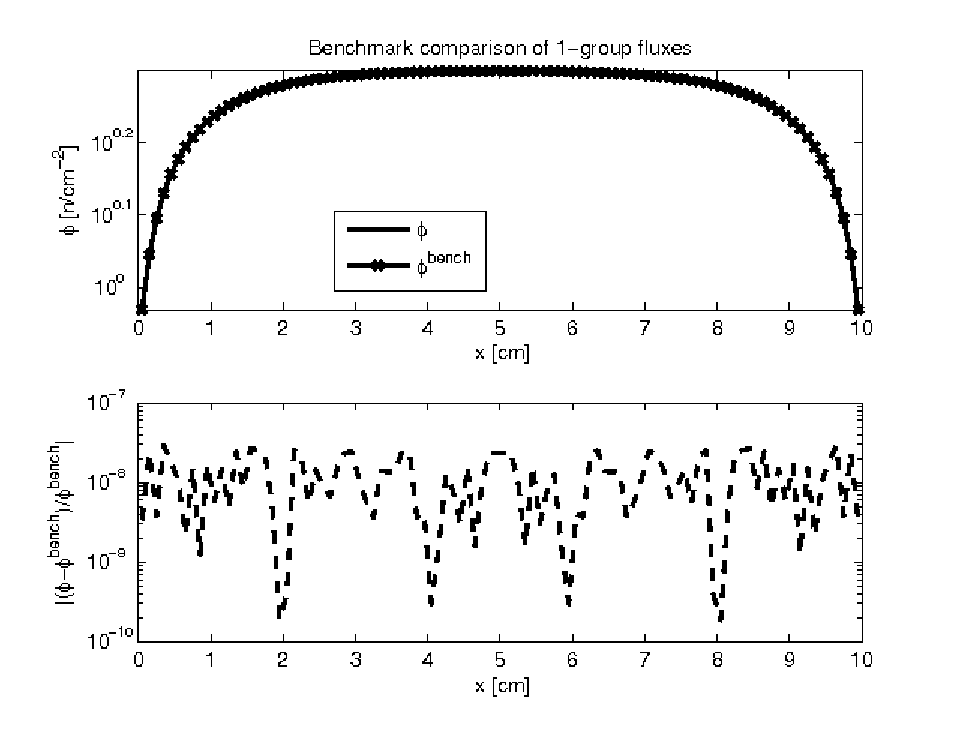
\includegraphics[keepaspectratio, width = 4.0 in]{one_d_comp}
      \caption{One-dimension, one-group sample problem.}
      \label{fig:one_d_comp}
  \end{figure}


  A second, two-dimensional problem was also solved.  This problem is a 10 cm by 10 cm square with vacuum boundaries.  The first 2 cm by 2 cm region contains a uniform isotropic source in the fast energy group (group 1).  In the 2 cm by 2 cm region diagonal and farthest from this source is a uniform isotropic source in the thermal group (group 2). The entire box is of uniform composition with the following data: $\Sigma_{T,1}=1.0$, $\Sigma_{s,1\to1}=0.3$, $\Sigma_{s,1\to2}=0.2$, $\Sigma_{T,2}=1.0$, and $\Sigma_{s,2\to2}=0.4$.  There is no transfer from group 2 to 1. Figure \ref{fig:two_d_comp} shows a comparison of the group-wise scalar flux down a main diagonal of the box (connecting the sources), along with the absolute value of the relative error with respect to the benchmark, and Figure  \ref{fig:two_d_flux} shows a contour plot of the fluxes from the MATLAB code. What appear to be nonphysical oscillations in the flux are due to a well-known numerical artifact known as ``ray effects'' that can most easily be mitigated by higher angular orders \cite{lewis1993cmn}.  Here, the $S_4$ approximation (12 directions in 2-D), 100 spatial intervals per dimension, and a convergence criteria of $1\times 10^{-9}$ were used.

  \begin{figure}[ht] 
      \centering
      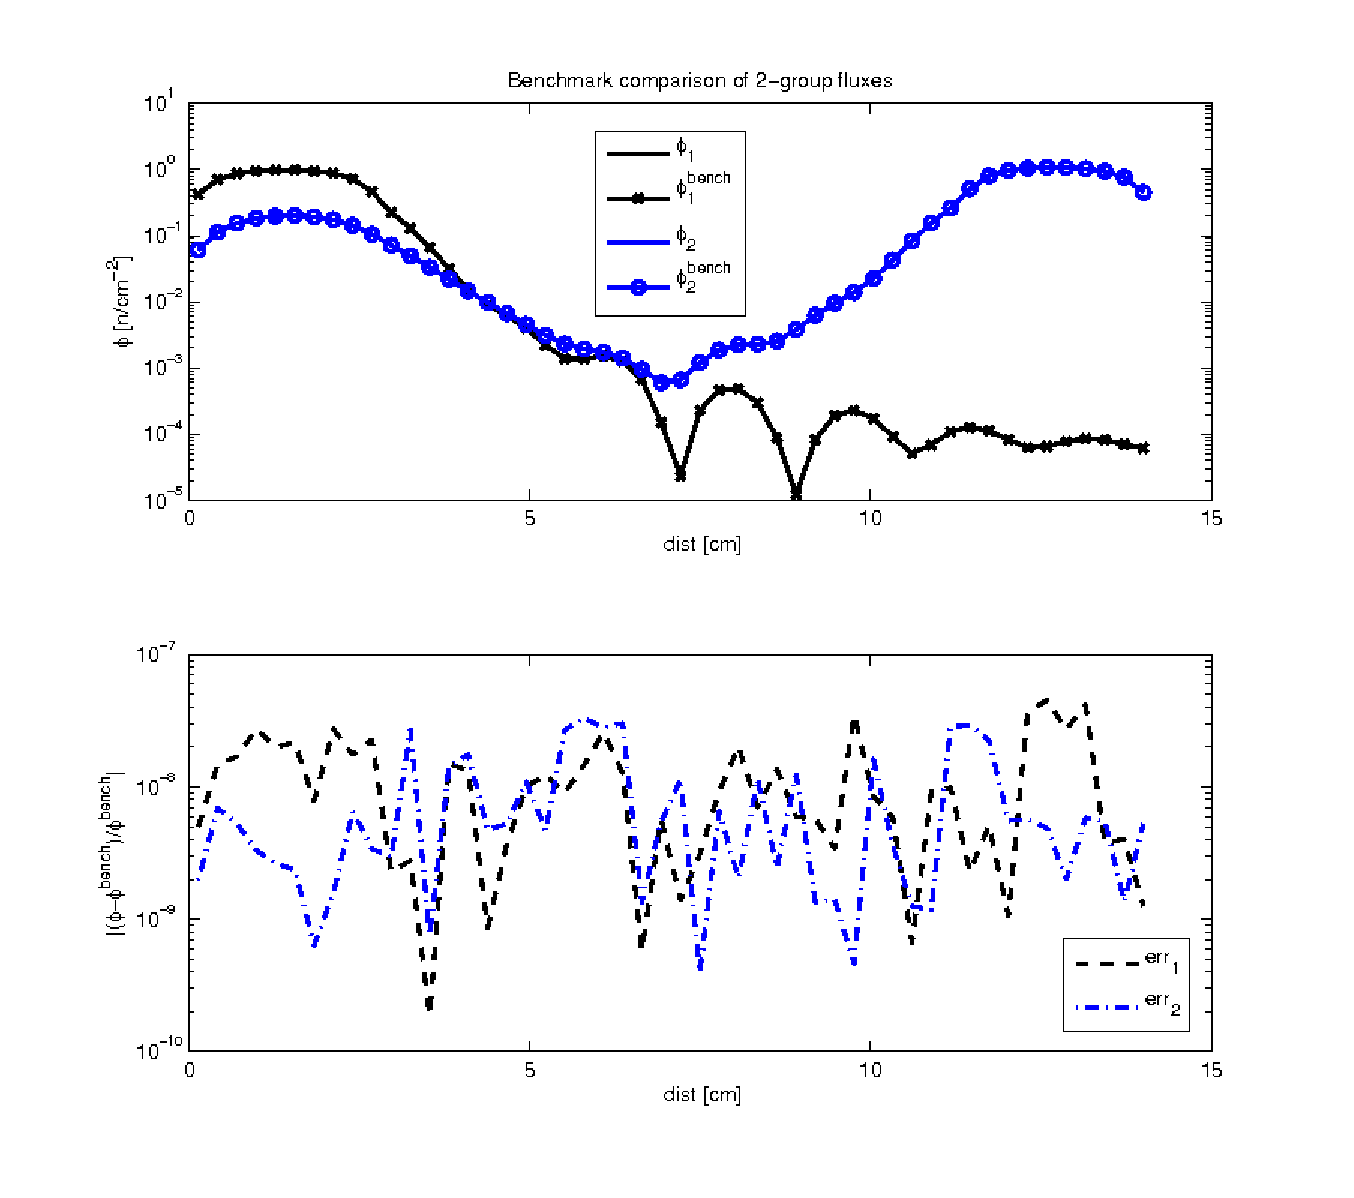
\includegraphics[keepaspectratio, width = 3.5 in]{two_d_comp}
      \caption{Two-dimensional, two-group sample problem comparison.}
      \label{fig:two_d_comp}
  \end{figure}

  \begin{figure}[ht]  
      \centering
      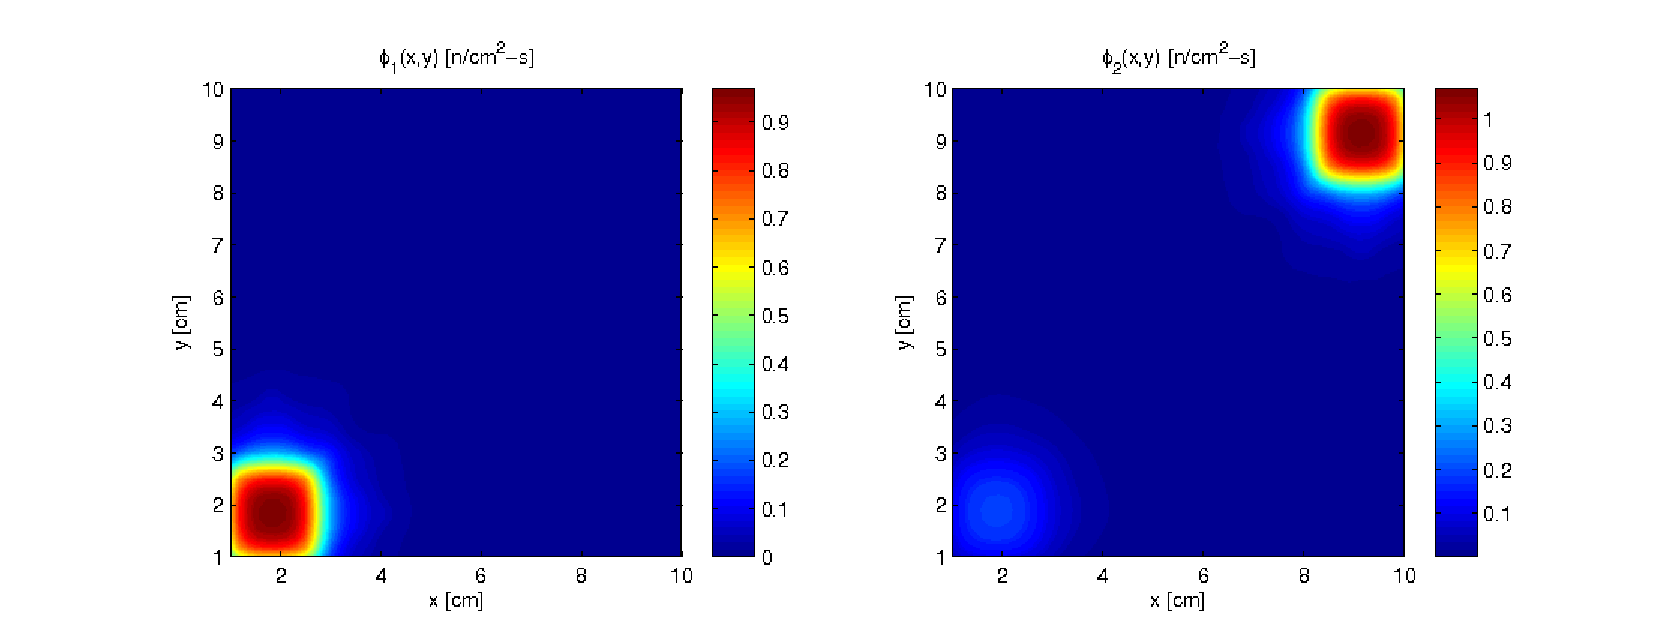
\includegraphics[keepaspectratio, width = 5.0 in]{two_d_flux}
      \caption{Two-dimensional, two-group sample problem fluxes.}
      \label{fig:two_d_flux}
  \end{figure}

  For both problems the error is small.  Moreover, the flux output from PARTISN is truncated at 8 decimals, which agrees well with the error observed.  In summary, the methods developed and implemented achieve the same solution as a production code, providing a solid base from which to approach a new method for solving the equations.

\section{Direct Solution Approach}
     The power iteration method using transport sweeps is very memory efficient, since at any given iteration, only the Legendre moments (or in the case of isotropic scattering and sources, just the scalar flux) are required along with the adjacent $\psi$ values. 

     The method can also be cast into matrix form.  For a simple problem with a uniform medium, two spatial cells, and two ordinates, $\psi_{i\pm1/2,n} = \alpha_{i,n} \psi_{i\mp1/2,n} + \beta_{i,n} Q_{i,n}$ becomes
	\begin{equation}
	\left
	[\begin{array}{cccccc}
	      1    &    0      &    0    &    0      &    0     &    0    \\
	  -\alpha  &    1      &    0    &    0      &    0     &    0    \\
	      0    &  -\alpha  &    1    &    0      &    0     &    0    \\
	      0    &    0      &    0    &    1      &    0     &    0    \\
	      0    &    0      &    0    & -\alpha   &    1     &    0    \\
	      0    &    0      &    0    &    0      &  -\alpha &    1    \\
	\end{array} 
	\right ] 
	\left
	[\begin{array}{c}
	  \psi_{1/2,2}     \\
	  \psi_{3/2,2}     \\
	  \psi_{5/2,2}     \\
	  \psi_{5/2,1}     \\
	  \psi_{3/2,1}     \\
	  \psi_{1/2,1}     \\
	\end{array} 
	\right ] =
	\left
	[\begin{array}{c}
	  \psi_{L}       \\
	  \beta Q_{1,2}  \\
	  \beta Q_{2,2}  \\
	  \psi_{R}       \\
	  \beta Q_{2,1}  \\
	  \beta Q_{1,1}  \\
	\end{array} 
	\right ] \, ,
	\end{equation}
  or $\bm{L\psi} = \bm{Q}$.  For the power iteration approach, the right hand side is guessed, and the iterations are $\bm{\psi}^{l+1}=\bm{L}^{-1}\bm{Q}^l$.

  Unfortunately, the PI method is extremely ineffective when the problem is highly diffusive, \ie when the ratio $\Sigma_S/\Sigma_T$ is large.  This can be explained readily via a physical interpretation.  If the initial scattering source (the $\psi$ component of $Q$) is set to zero, then the right hand side is just the external source.  After one iteration and update, all particles having collided once are included in the scattering term, and after $N$ iterations $N$th-collided particles are included.  For a problem with high scattering, particles on average have collided many times, and consequently, many iterations are required to reflect that fact.

   To move away from the limitations of PI, many acceleration techniques have been developed over time, but they are often difficult to implement.  As an alternative approach, it is possible to remove iterations on scattering altogether by moving all $\psi$ terms to the left hand side of the equations.  To illustrate using the above example, we find after some permutations
    {\small
    \begin{equation}
    \begin{split}
    \left
    [\begin{array}{cccccc}
    1-\gamma   &  -\gamma        & -\alpha-\gamma  &  -\gamma       &  0              &  0  \\
	    0  &       1         &  0              &  0             &  0              &  0  \\
	    0  &       0         & 1-\gamma        & -\gamma        & -\alpha-\gamma  & -\gamma \\
    -\gamma    & -\alpha-\gamma  &  -\gamma        & 1-\gamma       &  0              &  0  \\
	    0  &  0              &  0              &  0             &  1              &  0  \\
	    0  &  0              &  -\gamma        & -\alpha-\gamma &  -\gamma        & 1-\gamma   \\
    \end{array} 
    \right ]
    \times \left
    [\begin{array}{c}
      \psi_{1/2,1}     \\
      \psi_{1/2,2}     \\
      \psi_{3/2,1}     \\
      \psi_{3/2,2}     \\
      \psi_{5/2,1}     \\
      \psi_{5/2,2}     \\
    \end{array} 
    \right ] = 
    \left
    [\begin{array}{c}
      \beta S    \\
      \psi_{L}    \\
      \beta S    \\
      \beta S    \\
      \psi_{R}    \\
      \beta S    \\
    \end{array} 
    \right ] \, 
    \end{split}
    \label{eq:simp_matx} 
    \end{equation}
    }
    where  $\gamma = w \beta \frac{\Sigma_S}{2}\frac{1}{2}$ since $Q_{i,n} = w \frac{\Sigma_S}{2}\frac{1}{2}(\psi_{i+1/2,1}+\psi_{i-1/2,1}+\psi_{i+1/2,2}+\psi_{i-1/2,2})+S$.

    For arbitrary multigroup problems in 1-D and 2-D, a code was written in MATLAB to construct the matrices akin to that of Eq. \ref{eq:simp_matx}.  Diagonals are constructed, and a sparse matrix is produced via the {\sf spdiags()} command. 

    The structure of the matrix is related directly to the quadrature order $N$ and number of groups $G$.  For 1-D problems, the matrix bandwidth is $BW=2GN$, and the resulting structure matches what can be found in the literature\cite{patton2002apg}. For 2-D problems (for which no reference structure was found in the literature), the matrix is ordered by rows of horizontal and vertical edge fluxes and the bandwidth is $BW=W=2GN(n_x+1)$, where $n_x$ is the number of $x$ divisions.  Other ordering schemes are possible, but the one used is straightforward and maintains bandwidth characteristics similar to the one-dimensional case.  Figures \ref{fig:lalala} and \ref{fig:two_d_matx_full} show the resulting matrices for sample 1-D and 2-D problems, respectively.


    \begin{figure}[ht]
      \centering
	\subfigure[full matrix]{
	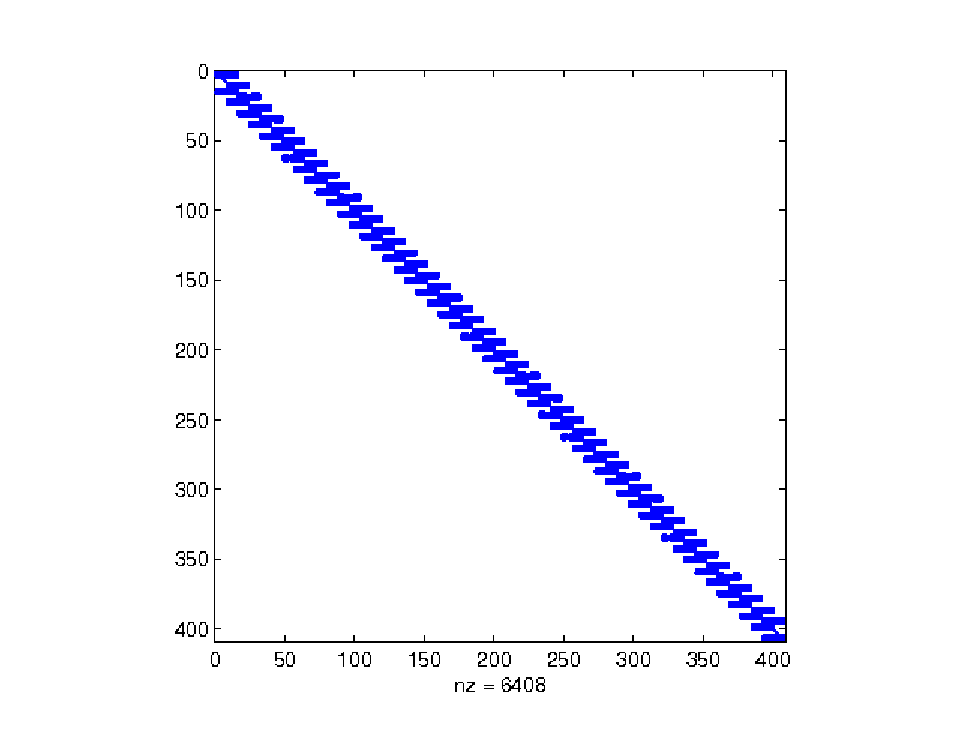
\includegraphics[keepaspectratio, width = 3.0 in]{one_d_matx_full}
	}
	\subfigure[zoomed]{
	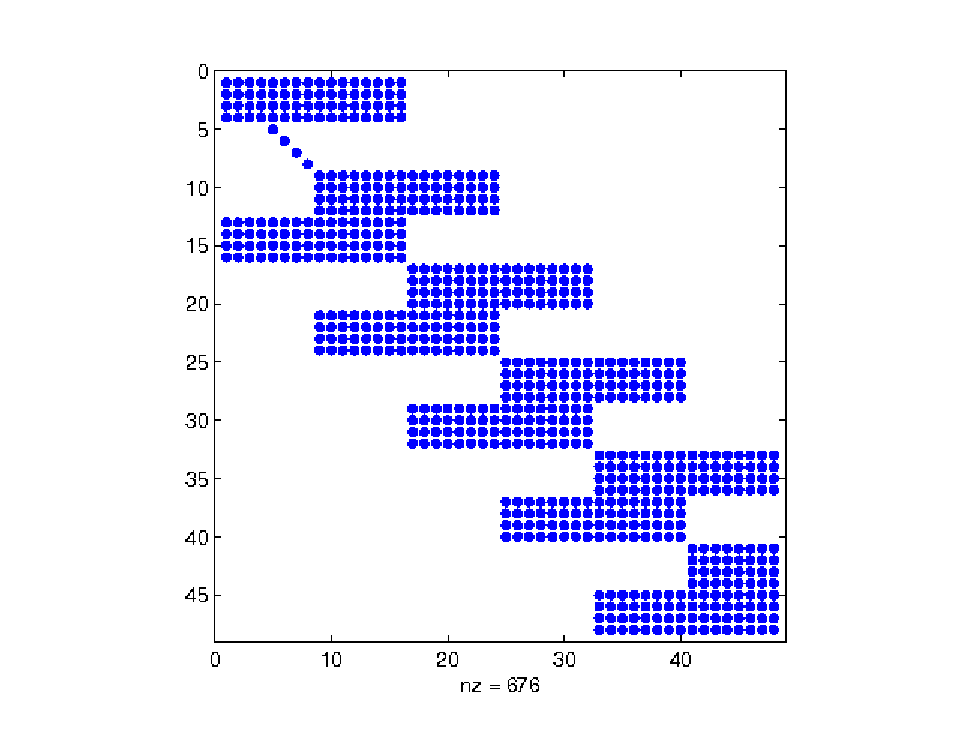
\includegraphics[keepaspectratio, width = 3.0 in]{one_d_matx_zoom}
	}
      \caption{1-D, 1-G, 50 mesh, S$_8$, $BW=2GN=16$, $(50+1)\cdot1\cdot 8=408$ unknowns.}
      \label{fig:lalala}
    \end{figure}

%   \begin{figure}[ht]  
%       \centering
%       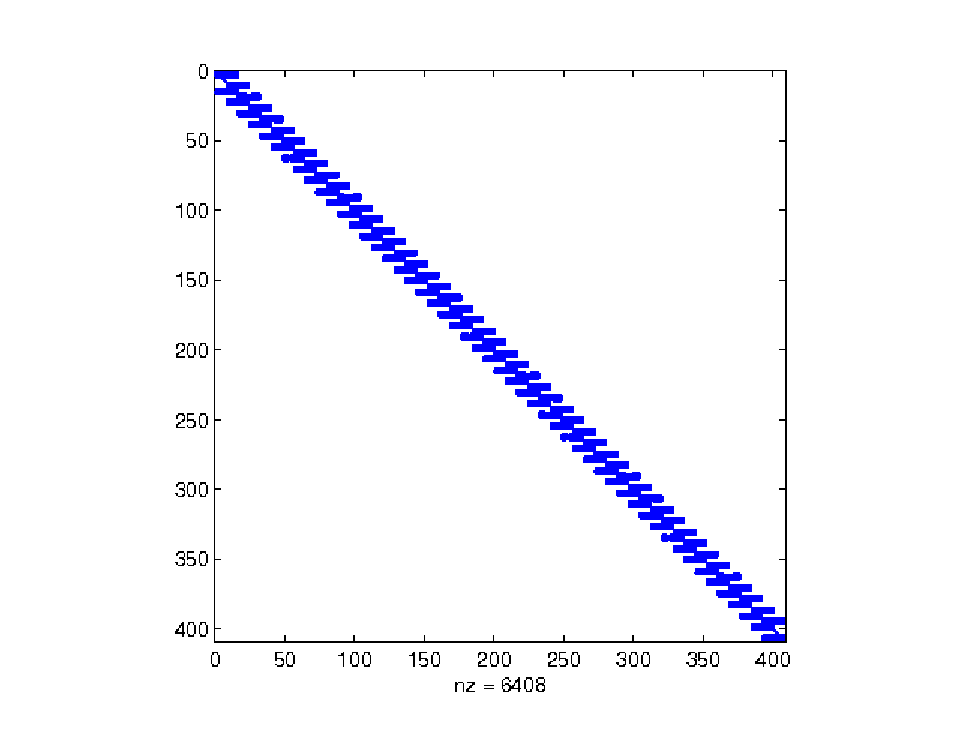
\includegraphics[keepaspectratio, width = 4.0 in]{one_d_matx_full}
%       \caption{1-D, 1-G, 50 mesh, S$_8$, $BW=2GN=16$, $(50+1)\cdot1\cdot 8=408$ unknowns.}
%       \label{fig:lalala}
%   \end{figure}
% 
%   \begin{figure}[ht]  
%       \centering
%       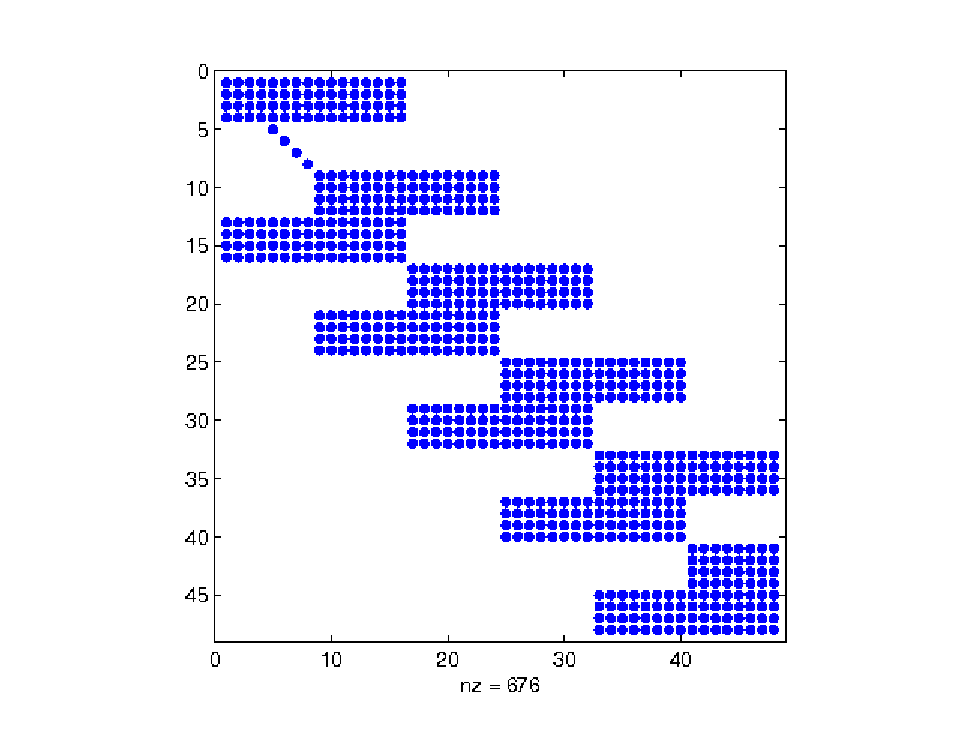
\includegraphics[keepaspectratio, width = 4.0 in]{one_d_matx_zoom}
%       \caption{Zoom of the previous.}
%   \end{figure}
    \begin{figure}[ht]
      \centering
	\subfigure[full matrix]{
	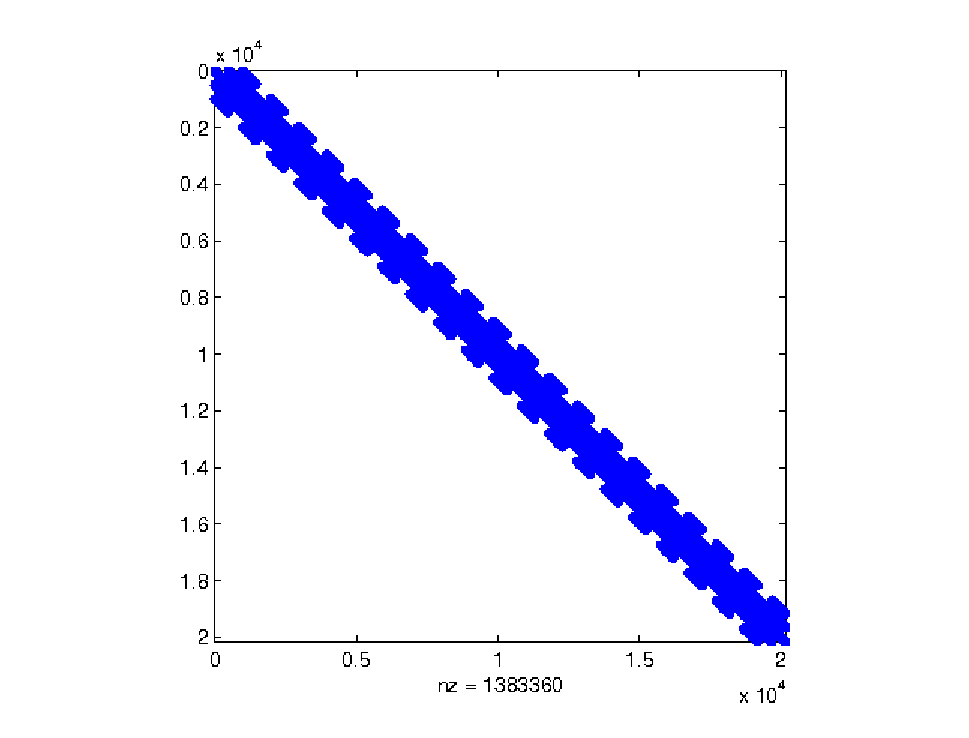
\includegraphics[keepaspectratio, width = 3.0 in]{two_d_matx_full}
	}
	\subfigure[similar to (a), and zoomed]{
	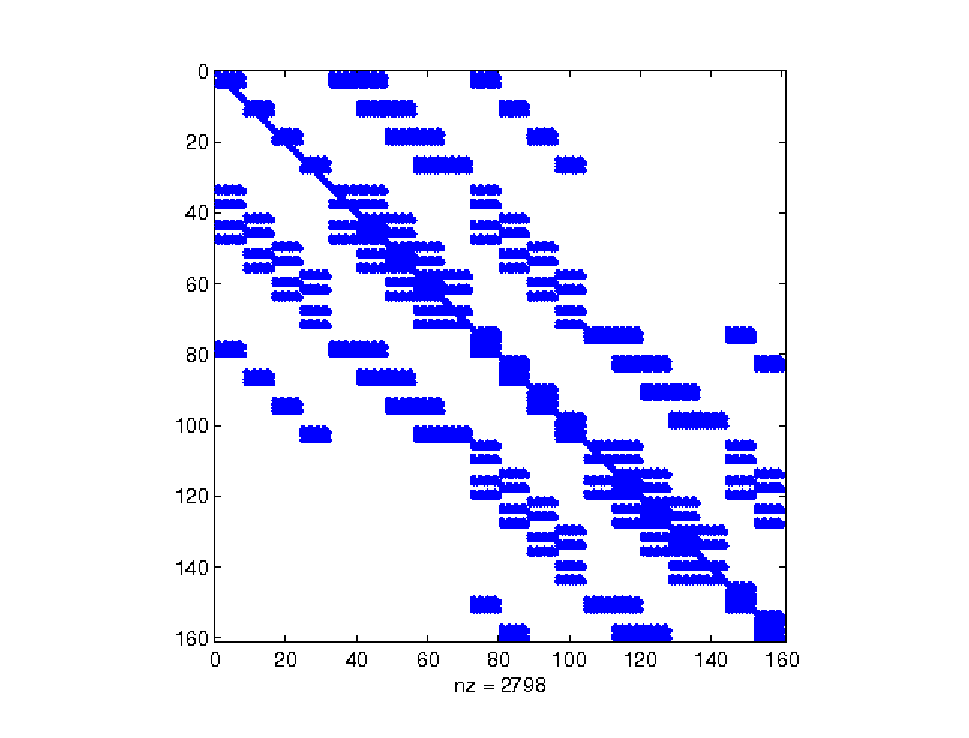
\includegraphics[keepaspectratio, width = 3.0 in]{two_d_matx_zoom}
	}
      \caption{2-D, 2-G, 20 $\times$ 20 mesh, S$_4$, $BW=2GN(nx+1)=1008$, $((20+1)(20)+(20)(20+1))\cdot2\cdot2=20160$ unknowns (shown in (a)).}
      \label{fig:two_d_matx_full}
    \end{figure}

%   \begin{figure}[ht]  
%       \centering
%       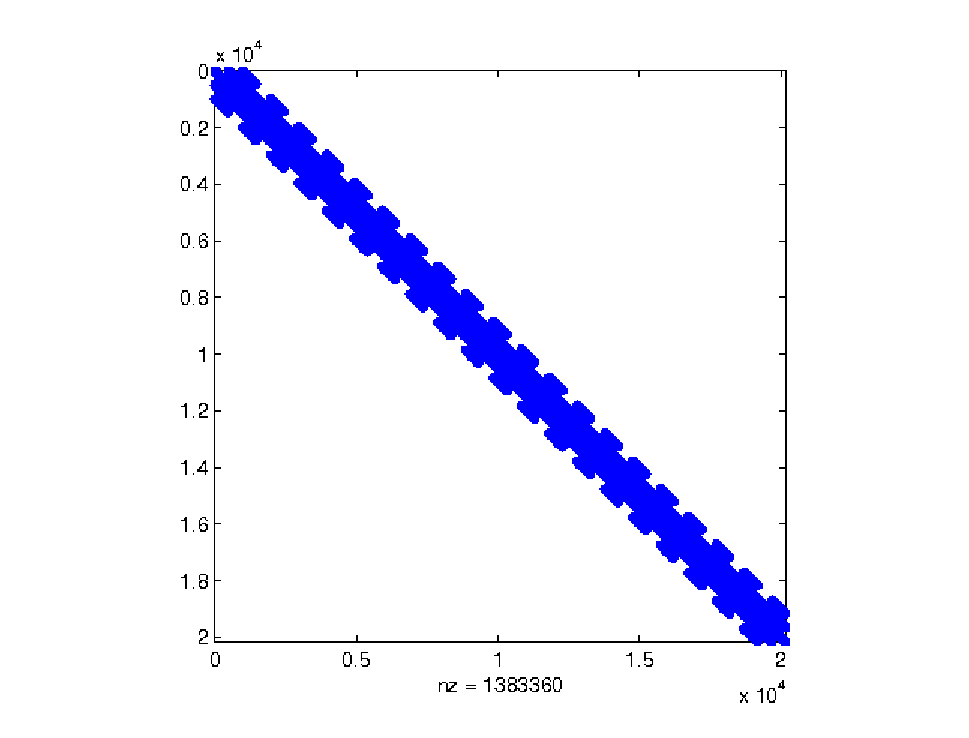
\includegraphics[keepaspectratio, width = 4.0 in]{two_d_matx_full}
%       \caption{2-D, 2-G, 20 $\times$ 20 mesh, S$_4$, $BW=2GN(nx+1)=1008$, $((20+1)(20)+(20)(20+1))\cdot2\cdot2=20160$ unknowns.}
%   \end{figure}
% 
%   \begin{figure}[ht]  
%       \centering
%       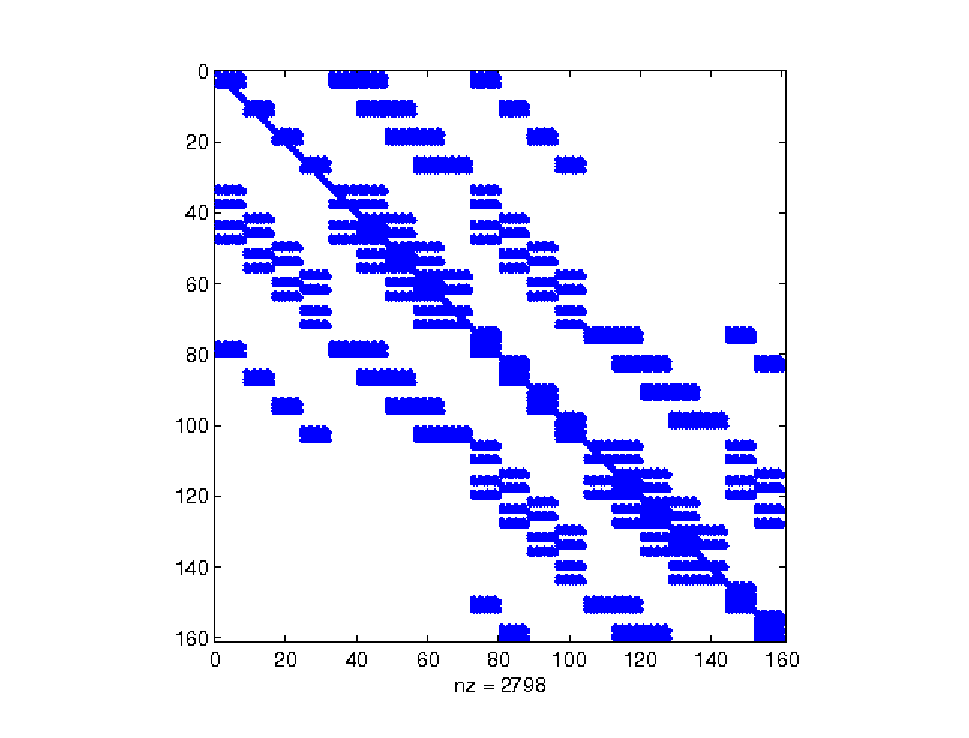
\includegraphics[keepaspectratio, width = 4.0 in]{two_d_matx_zoom}
%       \caption{Similar to last, but zoomed.}
%   \end{figure}

\section{Results}

  In this section, we present results for several simple one-dimensional, one-group, homogeneous problems with isotropic source and scatter.  The materials are the same as the one-dimensional problem above, except for the third case which varies $\Sigma_S/\Sigma_T$ between 0 and 1, keeping the original $\Sigma_T$ constant.  More complicated problems (\ie heterogeneous, multigroup, and 2-D) could be analyzed, but the problems investigated here already give a strong indication of the costs and benefits of the method.

  For all problems, the standard power iteration method with sweeps was used.  Additionally, Gaussian elimination by way of MATLAB's ``backslash'' command is used.  Finally, both GMRES(4) (\ie GMRES with restarts after 4 iterations) and BiCG-STAB were each used in conjunction with an ILU(0) and ILU(tp) (with a drop tolerance of $1\cdot10^{-4}$) preconditioner.  For PI and the Krylov solvers, a convergence criteria of $1\times 10^{-6}$ was used following the literature \cite{patton2002apg}.  It must be noted that the computational times listed below are then coupled to the given convergence criteria; for less stringent criteria, the iterative schemes would become more attractive and {\it vice versa} for a smaller criteria.
 
\subsection{Effect of Mesh Count}

  The first problem investigated the impact a large number of spatial meshes has on the various methods.  The computational time as a function of mesh size is shown in Figure \ref{fig:one_d_mesh_study} for each of the methods (total time), the preconditioner construction, and the matrix construction.  The direct methods are all significantly faster than the PI method; notably, elimination is the fastest method and is nearly twice as fast as PI.  Moreover, the ILU(0) preconditioner is most efficient, and BiCG-STAB outperforms GMRES(4).

  The general trend for all cases is linear.  For the direct approach, this makes sense; since the matrix bandwidth does not increase, the matrix and preconditioner construction times should be linear with the size as should be the Krylov solver times.  These trends have been previously observed in the literature \cite{patton2002apg}.

  \begin{figure}[!]  
      \centering
      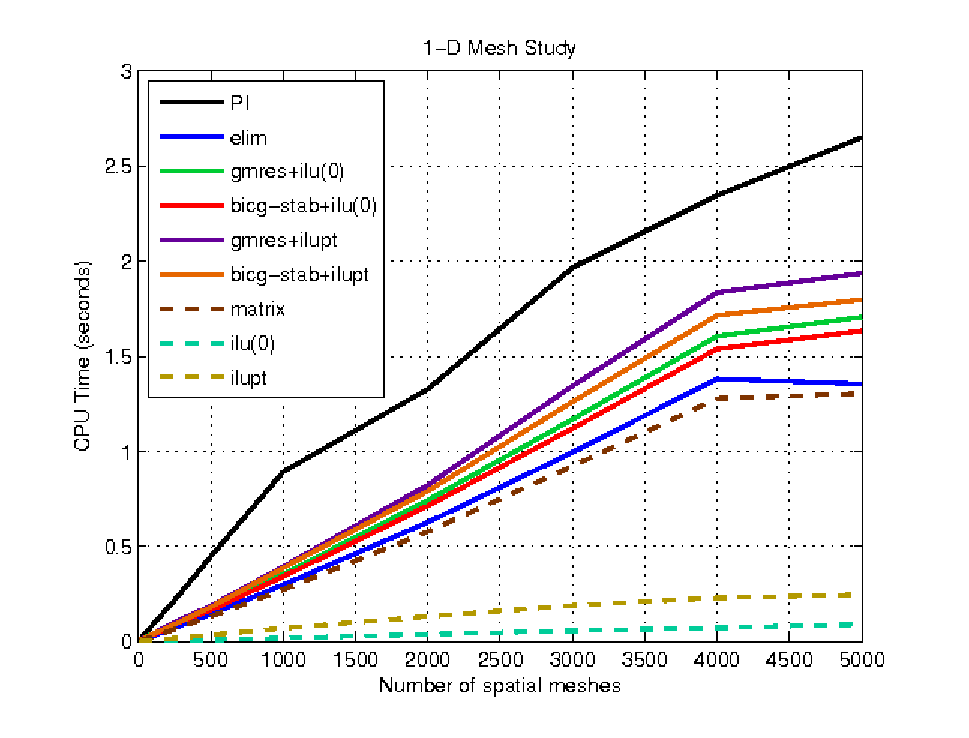
\includegraphics[keepaspectratio, width = 4.5 in]{one_d_mesh_study}
      \caption{$S_8$, varying mesh}
      \label{fig:one_d_mesh_study}
  \end{figure}

\subsection{Effect of Angular Order}
  The second study investigated the effect of larger quadrature orders.  The computational time for $S_N$ orders of 2, 4, 8, 16, and 32 for a problem of 2000 meshes is provided in Figure \ref{fig:one_d_sn_study}.  Here, we find a nonlinear dependence on the order, and this makes sense\cite{patton2002apg}.  Since the bandwidth is $2GN$, an increase in $N$ by a factor of 2 increases the number of nonzero matrix entries by $2^2$.  Thus, the matrix construction time, which comprises the bulk of the direct approaches, should also scale roughly as $N^2$.  Moreover, the ILU times and subsequent Krylov iterations are also affected, though it is hard to say what the effect is beyond being nonlinear.

  Beyond $N=8$, the matrix construction time takes so long that the direct approach becomes less efficient than the PI approach.  Consequently, a way to minimize this cost is needed.  It should be noted that the matrix construction time is not discussed in the the literature reviewed.  This likely suggests that the libraries used (SPARSKIT, in the case of Patton and Holloway \cite{patton2002apg}) are much more efficient then MATLAB's utilities.
  
  \begin{figure}[!]  
      \centering
      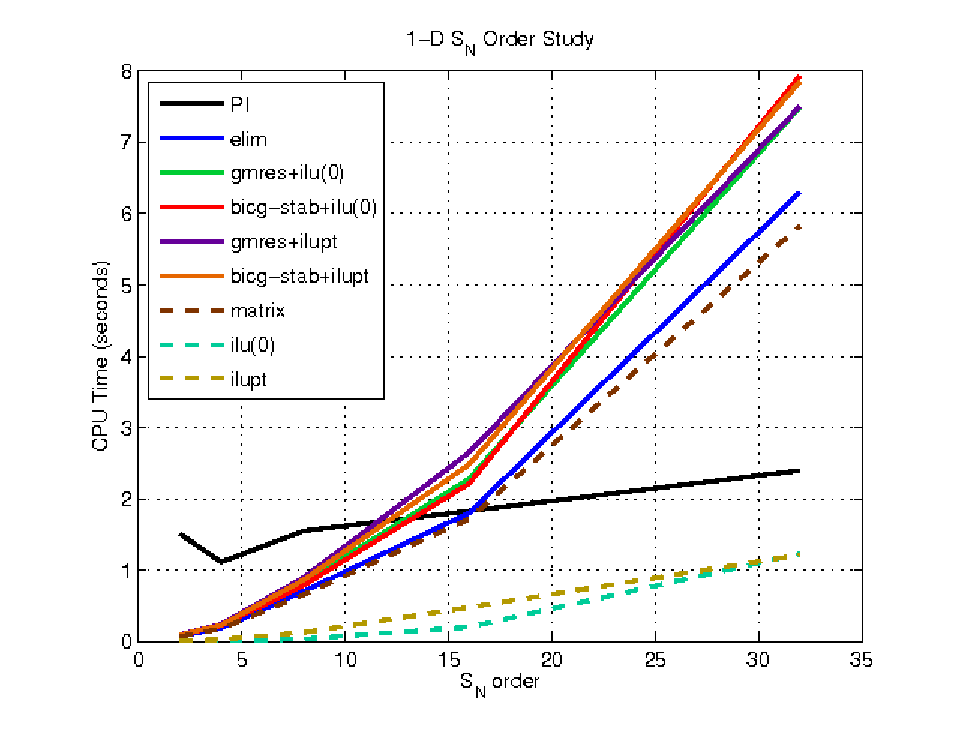
\includegraphics[keepaspectratio, width = 4.5 in]{one_d_sn_study}
      \caption{2000 mesh, varying $S_N$ order.}
      \label{fig:one_d_sn_study}
  \end{figure}

\subsection{Effect of Scattering Ratio}

  A final example investigated the impact of the scattering ratio $\Sigma_S/\Sigma_T$ on the solvers.  The computational time as a function of $\Sigma_S/\Sigma_T$ is shown in Figure \ref{fig:one_d_sigs_study}.  The striking feature of the plot is the rapid rise in PI computation time for large scattering ratios.  Contrarily, all the direct solver and construction times are essentially constant, and hence, a direct approach should be a viable alternative for highly diffusive problems.

  \begin{figure}[!]  
      \centering
      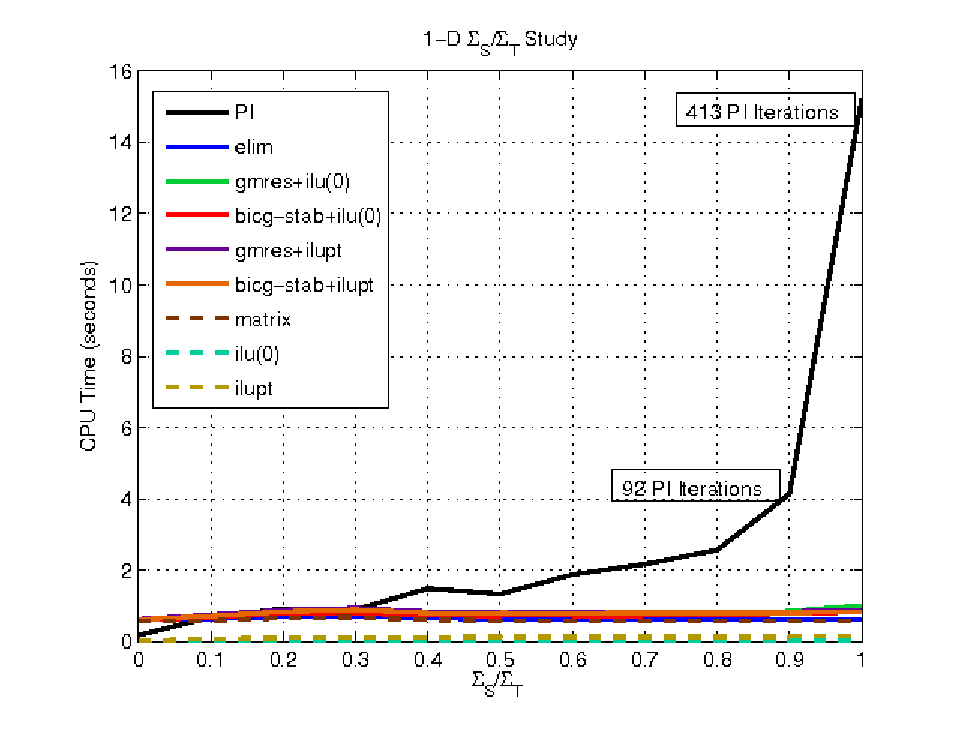
\includegraphics[keepaspectratio, width = 4.5 in]{one_d_sigs_study}
      \caption{1000 mesh, $S_8$, $\Sigma_S/\Sigma_T \in [0,1]$.}
      \label{fig:one_d_sigs_study}
  \end{figure}

\section{Conclusion}

In summary, this paper has presented the discrete ordinates method and a way to solve the resulting equations directly.  The standard PI approach and the direct approach were implemented in MATLAB and verified against a production code.  Several one-dimensional, monoenergetic problems were investigated to compare the PI method to direct approach coupled with various solvers.  

For the problems studied, no test case was solved more quickly via a Krylov method than elimination.  This suggests two things. First, MATLAB has very highly optimized procedures for performing elimination.  Second, more work should be done to investigate potential preconditioners.  Moreover, the matrix construction time comprised most of the total direct solution times, and 90\% of the construction time was spent in the MATLAB {\sf spdiags()} command.  Likely, a move to a compiled language and high performance sparse libraries would show something different. Lastly, while the difference was relatively minimal, BiCG-STAB outperformed GMRES(4) for problems studied.

As a final note, an approach somewhat similar to the ones taken in this paper is of current interest at Oak Ridge National Laboratory (ORNL).  The code ``Denovo'' uses GMRES to solve the $S_N$ equations in each group\cite{peplow2009sot}.  Moreover, the approach it takes is highly adaptable to parallel computations, and the code developers have recently been awarded over ten million processor hours to run Denovo on ORNL's Jaguar, currently the fastest computer in the world\footnote{See http://www.nccs.gov/leadership-science/petascale-early-science/}.

\bibliographystyle{unsrt}
\bibliography{biblio}


\end{document}
